\section{Định lý Cơ bản của phép tính vi tích phân}

\subsection{Nguyên hàm}
Phép lấy nguyên hàm là phép toán ngược của phép lấy đạo hàm. Nếu $F$ là đạo hàm của $f$, ta nói $F$ là một \textbf{nguyên hàm} của $f$.

\begin{example}
    Vì $(x)' = 1$, hàm $F(x) = x$ là một nguyên hàm của hàm $f(x)=1$. Tương tự, vì $(x+5)'=1$, hàm $G(x) = x+5$ cũng là một nguyên hàm khác của $f$.
\end{example}

\begin{proposition}
    Nếu $F$ là một nguyên hàm của $f$ trên khoảng $(a,b)$, thì tất cả các nguyên hàm khác của $f$ trên khoảng đó đều có dạng $F(x) + C$, trong đó $C$ là một hằng số thực.
\end{proposition}
\begin{proof}
    Giả sử $G$ là một nguyên hàm bất kỳ khác của $f$. Khi đó, ta có $(F-G)' = F' - G' = f - f = 0$.
    Do đó, theo Hệ quả 4.1.13, hàm $F-G$ phải là một hàm hằng, tức là $F(x) - G(x) = C$ với mọi $x \in (a,b)$.
\end{proof}

Nếu hàm $f$ có nguyên hàm, tập hợp tất cả các nguyên hàm của $f$ được gọi là \textbf{tích phân bất định} của $f$, và được ký hiệu là
\[ \int f(x) \dd x. \]
Theo quy ước, ta thường viết tập hợp này dưới dạng:
\[ \int f(x) \dd x = F(x) + C, \]
trong đó $F$ là một nguyên hàm cụ thể của $f$ và $C$ đại diện cho một hằng số tùy ý.

\begin{example}
    Một số nguyên hàm cơ bản:
    \begin{enumerate}[label=(\alph*)]
        \item $\int k \dd x = kx + C$ (với $k$ là hằng số).
        \item $\int x^n \dd x = \dfrac{x^{n+1}}{n+1} + C$ (với $n \neq -1$).
        \item Từ $(\ln|x|)' = \dfrac{1}{x}$, ta có $\int \dfrac{1}{x} \dd x = \ln|x| + C$.
        \item $\int e^x \dd x = e^x + C$. Tổng quát hơn, $\int e^{kx} \dd x = \dfrac{1}{k}e^{kx} + C$ (với $k \neq 0$).
        \item $\int \dfrac{1}{\sqrt{1-x^2}} \dd x = \arcsin x + C$.
        \item $\int \dfrac{1}{1+x^2} \dd x = \arctan x + C$.
    \end{enumerate}
\end{example}

\begin{proposition}[Tính tuyến tính của nguyên hàm]
    Nếu $f$ và $g$ có nguyên hàm, thì $f+g$ và $k \cdot f$ (với $k$ là hằng số) cũng có nguyên hàm, và:
    \[ \int [f(x) + g(x)] \dd x = \int f(x) \dd x + \int g(x) \dd x \]
    \[ \int [k \cdot f(x)] \dd x = k \int f(x) \dd x \]
\end{proposition}

\begin{example}
    Áp dụng tính tuyến tính để tính nguyên hàm của một đa thức:
    \begin{align*}
        \int (6x^2 - 8x + 3) \dd x &= 6 \int x^2 \dd x - 8 \int x \dd x + \int 3 \dd x \\
        &= 6 \left(\frac{x^3}{3}\right) - 8 \left(\frac{x^2}{2}\right) + 3x + C \\
        &= 2x^3 - 4x^2 + 3x + C.
    \end{align*}
\end{example}

\subsection{Công thức Newton-Leibniz và Định lý Cơ bản}

Định lý sau đây thiết lập một cầu nối vô cùng quan trọng giữa hai nhánh chính của giải tích: phép tính vi phân và phép tính tích phân.

\begin{theorem}[Định lý Cơ bản của Phép tính Vi tích phân, Phần 1] \label{thm:FTC1}
    Nếu hàm $f$ liên tục trên đoạn $[a, b]$ thì hàm $F$ được định nghĩa bởi
    \[ F(x) = \int_{a}^{x} f(t) \dd t, \quad a \le x \le b \]
    là một nguyên hàm của $f$ trên $[a,b]$. Do đó,
    \begin{importantbox}
        \[ \dfrac{\dd}{\dd x} \int_{a}^{x} f(t) \dd t = f(x). \]
    \end{importantbox}
\end{theorem}

Định lý này khẳng định rằng mọi hàm liên tục đều có nguyên hàm. Nó cho thấy rằng phép lấy đạo hàm của một tích phân sẽ trả về hàm số ban đầu, chứng tỏ phép tính vi phân và tích phân là hai quá trình ngược nhau.

Về mặt hình học, Định lý \ref{thm:FTC1} có thể được giải thích một cách trực quan. Nếu $f \ge 0$, thì $F(x)$ biểu diễn diện tích miền dưới đồ thị của $f$ từ $a$ đến $x$. Phần diện tích tăng thêm khi $x$ tăng một lượng nhỏ $h$, tức $F(x+h) - F(x)$, có thể được xấp xỉ bằng diện tích của một hình chữ nhật có chiều cao $f(x)$ và chiều rộng $h$.
\[ F(x+h) - F(x) \approx f(x) \cdot h \implies \dfrac{F(x+h) - F(x)}{h} \approx f(x). \]
Khi $h \to 0$, phép xấp xỉ này trở nên chính xác và ta có $F'(x) = f(x)$.

\begin{figure}[H]
    \centering
    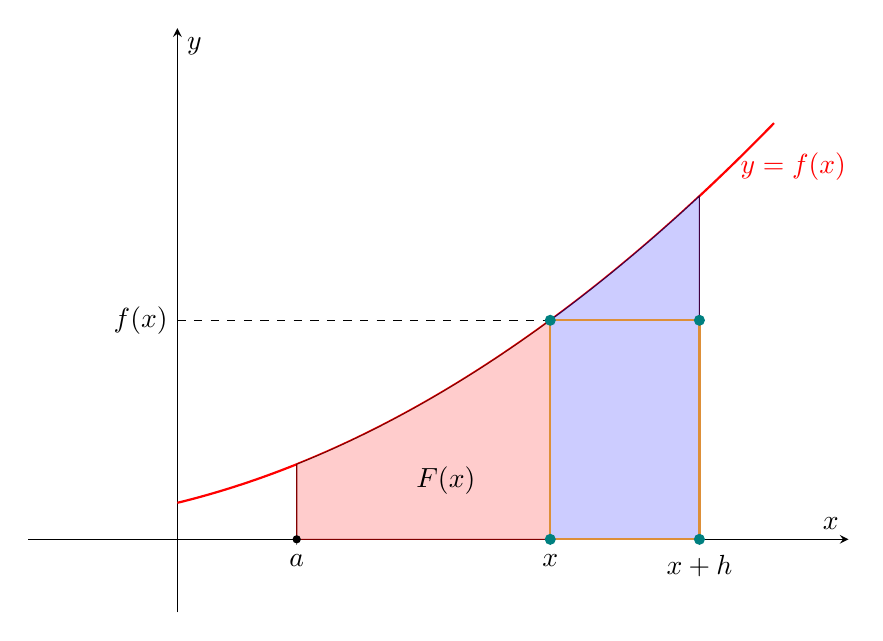
\begin{tikzpicture}
        \begin{axis}[
            axis lines=middle,
            xlabel=$x$,
            ylabel=$y$,
            xtick={0.8, 2.5, 3.5},
            xticklabels={$a$, $x$, $x+h$},
            ytick=\empty,
            xmin=-1, xmax=4.5,
            ymin=-1, ymax=7,
            width=12cm,
            height=9cm,
            clip=false,
            % Khai báo hàm f(x) để vẽ
            declare function={
                myfunc(\t) = 0.2*\t^2 + 0.5*\t + 0.5;
            }
        ]
        
        % Tọa độ các điểm chính
        \coordinate (a) at (axis cs:0.8,0);
        \coordinate (x) at (axis cs:2.5,0);
        \coordinate (x_h) at (axis cs:3.5,0);
        \coordinate (f_x) at (axis cs:2.5, {myfunc(2.5)});
        \coordinate (f_x_h) at (axis cs:3.5, {myfunc(3.5)});
        
        % 1. Vẽ đồ thị hàm số y=f(x)
        \addplot[
            domain=0:4, 
            samples=100, 
            color=red, 
            thick
        ] {myfunc(x)} node[pos=0.9, right] {$y=f(x)$};
        
        % 2. Tô màu vùng F(x) (màu đỏ nhạt)
        \addplot[
            fill=red!20,
            draw=black!50!red,
            domain=0.8:2.5,
        ] {myfunc(x)} \closedcycle;
        \node at (axis cs:1.8, 0.8) {$F(x)$};
        
        % 3. Tô màu vùng F(x+h) - F(x) (màu xanh lá nhạt)
        \addplot[
            fill=blue!20,
            draw=black!50!violet,
            domain=2.5:3.5,
        ] {myfunc(x)} \closedcycle;

        % 4. Vẽ hình chữ nhật màu vàng bên trong vùng màu xanh
        \draw[thick, draw=yellow!50!purple] (axis cs:2.5,0) rectangle (axis cs:3.5, {myfunc(2.5)});

        % 5. Vẽ các đường gióng và nhãn
        % Đường gióng từ x tới f(x)
        \draw[dashed] (axis cs:0, {myfunc(2.5)}) node[left] {$f(x)$} -- (f_x);
        
        % Các điểm chấm trên đồ thị
        \fill[teal] (f_x) circle (2pt);
        % \fill[blue] (f_x_h) circle (2pt);
        \fill[teal] (axis cs:3.5, {myfunc(2.5)}) circle (2pt);
        
        % Các điểm chấm trên trục hoành
        \fill[teal] (x) circle (2pt);
        \fill[teal] (x_h) circle (2pt);
        \fill (a) circle (1.5pt);

        \end{axis}
    \end{tikzpicture}
    \caption{\centering Xấp xỉ tuyến tính của sự gia tăng diện tích. Diện tích của dải hẹp $\Delta F = F(x+h) - F(x)$ có giá trị gần bằng diện tích hình chữ nhật đáy $h$ và chiều cao $f(x)$.}
    \label{fig:fundamental-theorem-1}
\end{figure}

\begin{proof}
    Chứng minh dưới đây là cách hình thức hóa lý luận hình học ở trên. Theo định nghĩa đạo hàm, ta có:
    \[ F'(x) = \limit{h}{0} \dfrac{F(x+h) - F(x)}{h} = \limit{h}{0} \dfrac{1}{h} \int_{x}^{x+h} f(t) \dd t. \]
    Ta biến đổi biểu thức bên trong giới hạn:
    \[ \dfrac{1}{h} \int_{x}^{x+h} f(t) \dd t - f(x) = \dfrac{1}{h} \int_{x}^{x+h} [f(t) - f(x)] \dd t. \]
    Vì $f$ liên tục tại $x$, với mọi $\epsilon > 0$, tồn tại $\delta > 0$ sao cho nếu $|h| < \delta$ thì $|f(t) - f(x)| < \epsilon$ với mọi $t$ nằm giữa $x$ và $x+h$. Do đó:
    \[ \left| \dfrac{1}{h} \int_{x}^{x+h} [f(t) - f(x)] \dd t \right| \le \dfrac{1}{|h|} \int_{x}^{x+h} |f(t) - f(x)| \dd t < \dfrac{1}{|h|} |h| \epsilon = \epsilon. \]
    Điều này chứng tỏ $\limit{h}{0} \dfrac{1}{h} \int_{x}^{x+h} f(t) \dd t = f(x)$. Vậy $F'(x) = f(x)$.
\end{proof}

\begin{example}
    Áp dụng trực tiếp Định lý Cơ bản của Phép tính Vi tích phân:
    \[ \dfrac{\dd}{\dd x} \int_{0}^{x} t^2 \dd t = x^2. \]
\end{example}

\begin{example}
    Để tìm đạo hàm của $h(x) = \int_{1}^{\sqrt{x}} \dfrac{z^2}{z^4+1} \dd z$, ta sử dụng quy tắc chuỗi.
    Đặt $u = \sqrt{x}$ và $F(u) = \int_{1}^{u} \dfrac{z^2}{z^4+1} \dd z$.
    Khi đó $h(x) = F(u(x))$. Theo quy tắc chuỗi và Định lý \ref{thm:FTC1}:
    \[ h'(x) = F'(u) \cdot u'(x) = \dfrac{u^2}{u^4+1} \cdot \dfrac{1}{2\sqrt{x}} = \dfrac{(\sqrt{x})^2}{(\sqrt{x})^4+1} \cdot \dfrac{1}{2\sqrt{x}} = \dfrac{x}{x^2+1} \cdot \dfrac{1}{2\sqrt{x}}. \]
\end{example}

\begin{example}
    Xét một vật chuyển động thẳng với vận tốc tức thời tại thời điểm $t$ là $v(t)$. Quãng đường vật đi được từ thời điểm $a$ đến $t$ là $s(t) = \int_a^t v(u) \dd u$.
    Định lý Cơ bản của Phép tính Vi tích phân cho ta:
    \[ s'(t) = \dfrac{\dd}{\dd t} \int_a^t v(u) \dd u = v(t). \]
    Kết quả này hoàn toàn phù hợp với định nghĩa vật lý rằng vận tốc là đạo hàm của quãng đường (hay vị trí) theo thời gian.
\end{example}

\begin{example}
    Hàm \textbf{sai số} (error function), ký hiệu $\mathrm{erf}(x)$, là một hàm quan trọng trong xác suất và thống kê, được định nghĩa bằng một tích phân:
    \[ \mathrm{erf}(x) = \dfrac{2}{\sqrt{\pi}} \int_{0}^{x} e^{-t^2} \dd t. \]
    Theo Định lý Cơ bản, đạo hàm của nó là $\mathrm{erf}'(x) = \dfrac{2}{\sqrt{\pi}} e^{-x^2}$. Đồ thị của hàm $e^{-x^2}$ có dạng hình chuông (đường cong Gauss) kinh điển.
    
    \begin{figure}[H]
        \centering
        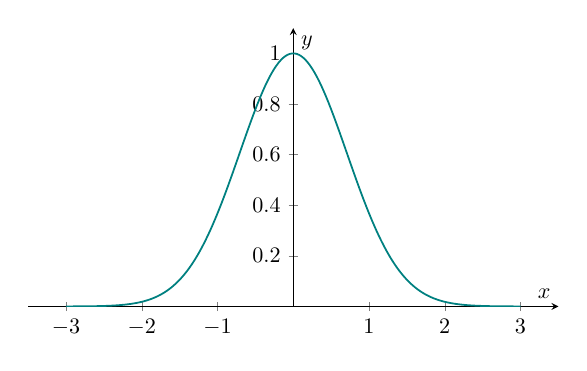
\begin{tikzpicture}[scale=0.8]
            \begin{axis}[
                axis lines=middle,
                samples=200,
                domain=-3:3,
                ytick={0.2, 0.4, 0.6, 0.8, 1.0},
                xmin=-3.5, xmax=3.5,
                ymin=0, ymax=1.1,
                xlabel=$x$,
                ylabel=$y$,
                width=10cm, height=6cm
            ]
            \addplot[color=teal, thick] {exp(-x^2)};
            \end{axis}
        \end{tikzpicture}
        \caption{Đồ thị hình chuông của hàm $e^{-x^2}$.}
    \end{figure}
\end{example}


\begin{theorem} (Công thức Newton-Leibniz)
    Nếu $f$ là hàm liên tục trên đoạn $[a, b]$ và $F$ là một nguyên hàm bất kỳ của $f$ trên đoạn đó, thì
    \begin{importantbox}
    \[ \int_{a}^{b} f(x) \dd x = F(b) - F(a) = \left.F(x)\right|_a^b. \]
    \end{importantbox}
\end{theorem}

Công thức Newton-Leibniz cung cấp một phương pháp vô cùng hiệu quả để tính tích phân xác định: thay vì phải tính giới hạn phức tạp của tổng Riemann, ta chỉ cần tìm một nguyên hàm của hàm số và tính hiệu các giá trị của nó tại hai đầu mút của đoạn tích phân.

Có thể giải thích gần đúng Công thức Newton-Leibniz bằng tổng Riemann như sau. Với bất kì phép chia nào của đoạn $[a, b]$ bởi $a = x_0 < x_1 < \dots < x_n = b$, vì
\[ F(x_i) - F(x_{i-1}) \approx F'(x_{i-1})(x_i - x_{i-1}) = f(x_{i-1})\Delta x_i \]
nên tổng Riemann tương ứng của hàm $f$ là
\[ \sum_{i=1}^{n} f(x_{i-1})\Delta x_i \approx \sum_{i=1}^{n} (F(x_i) - F(x_{i-1})) = F(x_n) - F(x_0) = F(b) - F(a). \]
Dẫn tới $\int_a^b f(x) \dd x \approx F(b) - F(a)$.

Một cách trực quan hơn, giả sử $a < b$ và $f \ge 0$. Ta dùng ý nghĩa tích phân $\int_a^b f(x) \dd x$ là diện tích bên dưới đồ thị của $f$ trên đoạn $[a, b]$, và lấy $F(x)$ là diện tích bên dưới đồ thị trên đoạn $[a, x]$. Khi đó, $F(a) = 0$ và $F(b)$ bằng diện tích trên toàn đoạn $[a, b]$, nên hiển nhiên $\int_a^b f(x) \dd x = F(b) - F(a)$. Từ Định lý Cơ bản của Phép tính Vi tích phân (Phần 1), ta đã biết $F$ là một nguyên hàm của $f$, và vì hai nguyên hàm bất kì của $f$ chỉ khác nhau một hằng số, nên để tính hiệu số $F(b) - F(a)$ ta dùng nguyên hàm nào cũng được. Đây cũng là nội dung của chứng minh bên dưới.

\begin{proof}
    Theo Định lý Cơ bản của Phép tính Vi tích phân (Phần 1) \ref{thm:FTC1}, hàm
    \[ G(x) = \int_a^x f(t) \dd t \]
    là một nguyên hàm của $f$. Ta có ngay $G(a) = \int_a^a f(t) \dd t = 0$, và
    \[ G(b) - G(a) = G(b) = \int_a^b f(t) \dd t. \]
    Bây giờ, giả sử $F$ là một nguyên hàm bất kỳ khác của $f$. Khi đó, tồn tại hằng số $C$ sao cho $F(x) = G(x) + C$ (theo Mệnh đề 5.2.2). Ta có:
    \[ F(b) - F(a) = (G(b)+C) - (G(a)+C) = G(b) - G(a) = \int_a^b f(t) \dd t. \]
    Điều này cho thấy kết quả không phụ thuộc vào việc chọn nguyên hàm cụ thể.
\end{proof}

\begin{example}
    Ta tính dễ dàng bằng Công thức Newton–Leibniz:
    \[ \int_{0}^{1} x \dd x = \left. \frac{1}{2}x^2 \right|_0^1 = \frac{1}{2}(1)^2 - \frac{1}{2}(0)^2 = \frac{1}{2}. \]
\end{example}

\begin{example}
    Tiếp tục Ví dụ 5.2.13, ta xét một vật chuyển động theo một chiều thẳng, với tốc độ tức thời tại thời điểm $t$ là $v(t)$ biến đổi liên tục. Chiều dài quãng đường đi được của vật từ thời điểm $a$ tới thời điểm $t$ cho bởi tích phân
    \[ s(t) = \int_a^t v(u) \dd u. \]
    Lấy một điểm nào đó trên đường làm điểm gốc, thì vị trí của xe ở thời điểm $t$ cho bởi số thực $x(t)$. Vì vận tốc là đạo hàm của vị trí theo thời gian, $v(t) = x'(t)$, nên Công thức Newton–Leibniz cho chiều dài quãng đường đi được của vật từ thời điểm $a$ tới thời điểm $t$ bằng
    \[ s(t) = \int_a^t v(u) \dd u = x(t) - x(a). \]
    Đây cũng chính là lượng thay đổi vị trí của chiếc xe (ta đang giả thiết vật chỉ di chuyển theo một chiều, không đổi chiều), và như vậy không phụ thuộc vào cách chọn điểm gốc. Ta cũng có $s(t) = x(t) - x(a)$ với mọi $t$, tức là chiều dài quãng đường đi được và vị trí chỉ sai khác một hằng số. Đặc biệt nếu tốc độ chuyển động là hằng $v$ (chuyển động thẳng đều) thì ta thu lại công thức quen thuộc $x(b) - x(a) = v(b - a)$, tức là chiều dài đường đi bằng tốc độ đi nhân thời gian đi.
\end{example}

% TODO: Sửa lại tham chiếu
\begin{figure}[H]
    \centering
    \begin{tikzpicture}
        % Dòng thời gian
        \draw[->, thick, blue!60] (-1,0) -- (11,0) node[right] {thời gian};
        \fill[blue!60] (3,0) circle (2pt) node[above] {$a$};
        \fill[blue!60] (6,0) circle (2pt) node[above] {$t$};
        \fill[blue!60] (7.8,0) circle (2pt) node[above] {$b$};

        % Dòng vị trí
        \draw[->, thick, orange!80!black] (-1,1) -- (11,1) node[right] {$x$};
        \fill[orange!80!black] (0,1) circle (2pt) node[above] {0};
        \fill[orange!80!black] (2,1) circle (2pt) node[above] {$x(a)$};
        \fill[orange!80!black] (6,1) circle (2pt) node[above] {$x(t)$};
        \fill[orange!80!black] (8.5,1) circle (2pt) node[above] {$x(b)$};

        % Chú thích quãng đường s(t)
        \draw[<->, thick, green!60!black] (2, 2) -- (6, 2) node[midway, above] {$s(t)$};
    \end{tikzpicture}
    \caption{Vị trí và quãng đường trong chuyển động thẳng một chiều.}
    \label{fig:position_distance_v2}
\end{figure}

Trong sách giáo khoa trung học [SGKTHPT], tích phân xác định thường được định nghĩa bằng Công thức Newton-Leibniz, tiện cho tính toán nhưng khó thấy được ý nghĩa và ứng dụng.

\subsection{Bài tập}

\begin{exercise}
    Tính các tích phân xác định sau:
    \begin{enumerate}[label=(\alph*)]
        \item $\int_{1}^{3} (\sqrt{x} - \frac{2}{\sqrt[3]{x^2}} + x) \dd x$.
        \item $\int_{-2}^{2} |x^2 - 1| \dd x$.
        \item $\int_{0}^{\pi} |\cos x| \dd x$.
        \item $\int_{-1}^{2} f(x) \dd x$ với $f(x) = \begin{cases} x^3, & \text{nếu } -1 \le x < 1, \\ x^4, & \text{nếu } 1 \le x \le 2. \end{cases}$
    \end{enumerate}
\end{exercise}

\begin{exercise}
    Sử dụng Định lý Cơ bản của Phép tính Vi tích phân để tìm đạo hàm của các hàm số sau:
    \begin{enumerate}[label=(\alph*)]
        \item $g(x) = \int_{2}^{x} \sqrt{1+t^4} \dd t$.
        \item $h(x) = \int_{x}^{10} \ln(z^2+1) \dd z$.
        \item $F(x) = \int_{1}^{x^3} \cos(t) \dd t$.
        \item $G(x) = \int_{\sin x}^{\cos x} (1+v^2)^{10} \dd v$.
    \end{enumerate}
\end{exercise}

\begin{exercise}
    Cho hàm số $f(x) = \int_{0}^{x^2} \ln(t^2 + e) \dd t$. Hãy tính $f'(1)$.
\end{exercise}

\begin{exercise}
    Bằng cách lấy đạo hàm vế phải, hãy chứng minh các công thức nguyên hàm sau:
    \begin{enumerate}[label=(\alph*)]
        \item \[\int \dfrac{1}{x^2 \sqrt{1 + x^2}} = - \dfrac{\sqrt{1 + x^2}}{x} + C\]. 
        \item \[\int \frac{1}{x \sqrt{1-x^2}} \dd x = -\ln\left(\frac{1+\sqrt{1-x^2}}{x}\right) + C\].
        \item \[\int \frac{x^2}{\sqrt{a^2-x^2}} \dd x = \frac{a^2}{2}\arcsin\left(\frac{x}{a}\right) - \frac{x}{2}\sqrt{a^2-x^2} + C\].
    \end{enumerate}
\end{exercise}

\begin{exercise}
    Tính giá trị của biểu thức tích phân lồng nhau sau:
    \[ \int_{0}^{1} \left( \int_{1}^{y} e^{x^2} \dd x \right) \dd y. \]
    (Gợi ý: Đặt $F(y) = \int_{1}^{y} e^{x^2} \dd x$ và sử dụng tích phân từng phần).
\end{exercise}

\begin{exercise}
    Khảo sát sự thay đổi của tích phân $I_n = \int_0^1 x^n \dd x$ khi số nguyên dương $n$ tăng. Hãy giải thích kết quả bằng cách phác họa đồ thị của hàm $y=x^n$ với một vài giá trị của $n$.
\end{exercise}

\begin{exercise}
    Một bể chứa ban đầu có 500 lít nước. Nước được bơm vào bể với tốc độ $v(t) = 200 - 8t$ (lít/phút), trong đó $t$ là thời gian tính bằng phút kể từ lúc bắt đầu bơm. Hỏi sau 10 phút, lượng nước trong bể là bao nhiêu?
\end{exercise}

\begin{exercise}
    Lưu lượng giao thông tại một nút giao thông được mô hình hóa bởi hàm $f(t) = -400t^2 + 2400t + 4000$ (xe/giờ), với $t=0$ tương ứng với 7 giờ sáng. Hãy tính tổng số xe đi qua nút giao này trong khoảng thời gian từ 8 giờ sáng ($t=1$) đến 10 giờ sáng ($t=3$).
\end{exercise}

\begin{exercise}
    Dòng chảy của một con sông mang theo bùn. Tốc độ lắng đọng của bùn tại một vị trí nhất định được cho bởi hàm $d(t) = 10 \sqrt{t} + \frac{t^2}{100}$ (kg/ngày), với $t$ là thời gian tính bằng ngày. Hãy tính tổng khối lượng bùn lắng đọng trong 100 ngày đầu tiên.
\end{exercise}

\begin{exercise}
    Công suất tiêu thụ điện của một nhà máy (tính bằng megawatt, MW) được mô hình hóa bởi hàm $P(t) = 2t^2 + 30$, với $t$ là số giờ kể từ 6 giờ sáng. Hãy tính tổng năng lượng điện (tính bằng megawatt-giờ) mà nhà máy tiêu thụ trong khoảng thời gian từ 8 giờ sáng ($t=2$) đến 4 giờ chiều ($t=10$).
\end{exercise}

\begin{exercise}
    Cho hàm số $f(x) = \int_{0}^{x} \frac{(t-4)^2 e^t}{\sqrt{t^2+9}} \dd t$, với $x \in [0, 5]$. Hãy xác định giá trị của $x$ để $f(x)$ đạt giá trị nhỏ nhất.
\end{exercise}
